\documentclass[11pt]{beamer}
\usetheme{Warsaw}
\usepackage[utf8]{inputenc}
\usepackage[russian]{babel}
\usepackage[OT1]{fontenc}
\usepackage{amsmath}
\usepackage{amsfonts}
\usepackage{amssymb}
\usepackage{graphicx}

\usepackage{qrcode}

\author{Генералов Даниил}
\title{Фрактальные гравировки}
%\setbeamercovered{transparent} 
%\setbeamertemplate{navigation symbols}{} 
%\logo{} 
%\institute{} 
%\date{} 
%\subject{} 
\begin{document}

\begin{frame}
\titlepage
\end{frame}


\begin{frame}{Что?}
\begin{itemize}
\item Программа, генерирующая G-code для гравировки фрактала Гильберта (можно реализовать другие).
\item Поддерживаются скругления и выпиливание правильного $n$-угольника (предпочтительно где $n \ge 6$, ибо баги)
\item Можно выпилить дырочку, чтобы сделать \textit{брелок для \textbf{ключей!!}}

\end{itemize}

\end{frame}

\begin{frame}{Зачем?}
\begin{LARGE}Потому что это \textit{прикольно!}\end{LARGE}

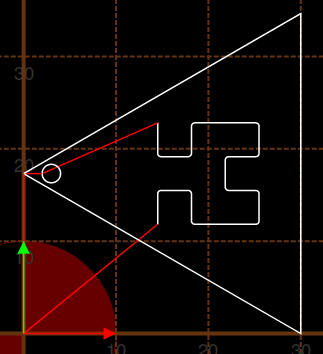
\includegraphics[scale=0.25]{trigon}
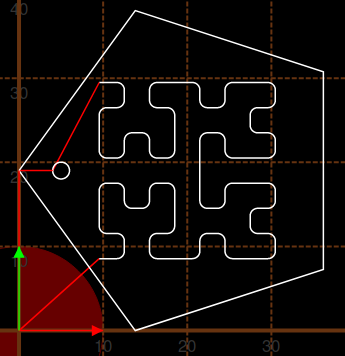
\includegraphics[scale=0.25]{5gon}
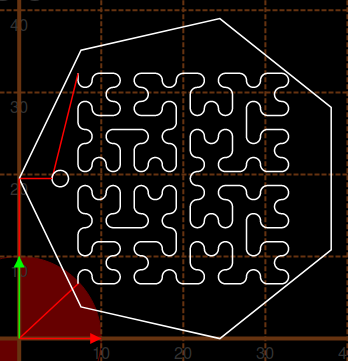
\includegraphics[scale=0.25]{7gon}

\begin{small}
(а ещё потому что преподы запросили)
\end{small}\begin{tiny}
(хотя и активно препятствовали работе)
\end{tiny}

\end{frame}
\begin{frame}{Как?}
\begin{itemize}
\item Фрактал -- знание определения + 2-летний стаж программирования черепашки
\item G-code -- методичка, опыт наблюдения за ЧПУ-станками и 3D-принтерами \item Скругления -- множественное эксперементальное биение головой об стену
\item $n$-угольный контур -- полярные координаты и много смещений и вращений и линейных превращений всего мира
\end{itemize}


\end{frame}

\begin{frame}{Как??}
\begin{enumerate}
\item Написал генератор фрактала
\item Написал переводчик в G-code
\item Добавил скруглятель углов
\item Понял, что значит ``контур многоугольником'' и добавил его
\item Добавил выпиливание отверстия
\item PROFIT!! \begin{tiny}(на самом деле еще нет)\end{tiny}
\end{enumerate}

\end{frame}

\begin{frame}{КАК?!?!?}

\begin{enumerate}
\item Получить координаты точек фрактала
\item Получить координаты углов $n$-угольника
\item Ужать фрактал, чтобы целиком помещался в $n$-угольнике
\item Скруглить углы хитрыми вычислениями
\item Выпилить фрактал
\item Выпилить отверстие
\item Выпилить контур
\end{enumerate}

\end{frame}

\begin{frame}{Когда?}
Когда никто не видит :)

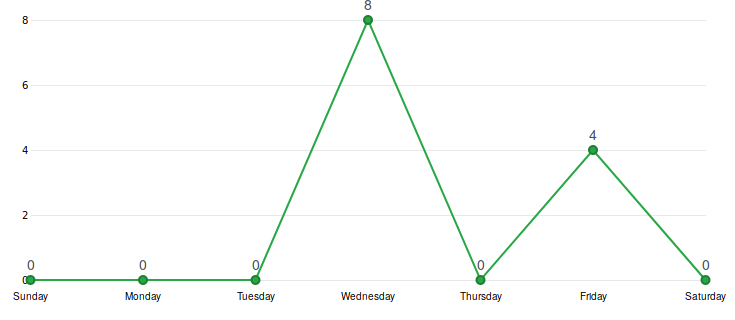
\includegraphics[scale=0.4]{code-graph}
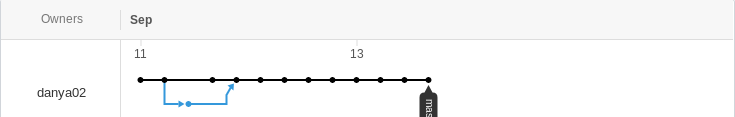
\includegraphics[scale=0.4]{code-network}
\end{frame}

\begin{frame}{Почему?}
Почему так некрасиво, почему такие баги, почему код такой неэффективный, ...

\begin{itemize}
\item Мало времени \begin{small}(и больше его не дают, насколько слёзно ты не просишь)\end{small}
\item Задержна коммуникации (техзадание не точное, но узнать про это можно только под конец)
\item Я не знаю геометрию (как определить точку центра самого большого вписанного квадрата и сторону этого квадрата?!)
\end{itemize}
\end{frame}

\begin{frame}{Где?}
На GitHub: \underline{https://github.com/danya02/hilbert-keychain}

\qrcode[height=2in]{https://github.com/danya02/hilbert-keychain}
\end{frame}
\begin{frame}{Доколе?}
\begin{center}
\begin{Huge}
Спасибо за внимание.
\end{Huge}
\end{center}
\begin{flushright}
\begin{Large}
-- Генералов Даниил
\end{Large}
\end{flushright}
\begin{center}
\qrcode[height=1in]{https://github.com/danya02/hilbert-keychain}

\end{center}
\end{frame}
\end{document}
